\documentclass[14pt]{beamer}

\usepackage[T1]{fontenc}
\usepackage{tikz}
\usepackage[quiet]{mathspec}
\usepackage{ifthen}

\usetikzlibrary{matrix,arrows.meta}


% Tells beamer that math mode should use serif fonts
\usefonttheme[onlymath]{serif}

% Sets the serif font (which is the main font)
\setmainfont{Linux Libertine O}

% Sets the font beamer uses, which is sans-serif by default
\setsansfont[
ItalicFont={Yanone Kaffeesatz Light},
Scale=1.3,
LetterSpace=2.0
]{Yanone Kaffeesatz Bold}

% Replaces every explicit \mathrm call to use this font
\setmathrm{Linux Libertine O}

% The base16 colour scheme?
\definecolor{sbase03}{HTML}{002B36}
\definecolor{sbase02}{HTML}{073642}
\definecolor{sbase01}{HTML}{586E75}
\definecolor{sbase00}{HTML}{657B83}
\definecolor{sbase0}{HTML}{839496}
\definecolor{sbase1}{HTML}{93A1A1}
\definecolor{sbase2}{HTML}{EEE8D5}
\definecolor{sbase3}{HTML}{FDF6E3}
\definecolor{syellow}{HTML}{B58900}
\definecolor{sorange}{HTML}{CB4B16}
\definecolor{sred}{HTML}{DC322F}
\definecolor{smagenta}{HTML}{D33682}
\definecolor{sviolet}{HTML}{6C71C4}
\definecolor{sblue}{HTML}{268BD2}
\definecolor{scyan}{HTML}{2AA198}
\definecolor{sgreen}{HTML}{859900}

\definecolor{Tropiteal}{RGB}{0,168,198}
\definecolor{TealDrop}{RGB}{64,192,203}
\definecolor{WhiteTrash}{RGB}{249,242,231}
\definecolor{AtomicBikini}{RGB}{174,226,57}
\definecolor{FeebleWeek}{RGB}{143,190,0}
\definecolor{ICantExpress}{RGB}{28,20,13}
\definecolor{Marty}{RGB}{250,42,0}

\colorlet{ColourBase}{Tropiteal}
\colorlet{ColourHl1}{Marty}
\colorlet{ColourHl2}{FeebleWeek}
\colorlet{ColourHl3}{TealDrop}
\colorlet{ColourDark}{ICantExpress}
\colorlet{ColourDark2}{Tropiteal}


\usetheme{metropolis}

\setbeamercolor{alerted text}{%
  fg=bazelGreen
}

\setbeamercolor{example text}{%
  fg=mLightBrown
}

\setbeamercolor{frametitle}{%
  use=normal text,
  fg=normal text.bg,
  bg=bazelGreen
}

\lstset{%
  basicstyle=\ttfamily\lst@ifdisplaystyle\fontsize{9pt}{9pt}\selectfont\fi,
  keywordstyle=\color{sgreen}, identifierstyle=\color{sblue}, 
  commentstyle=\color{sbase1}, stringstyle=\color{sorange},
  numberstyle=\color{sviolet}, showstringspaces=false,  
  breaklines=true,
  tabsize=5,
}

\lstalias[]{gnumake}[gnu]{make}




\usetikzlibrary{fadings,decorations.pathmorphing}
% Code courtesy of https://tex.stackexchange.com/a/137438/39313

\makeatletter
\newif\iftikz@shading@path

\tikzset{
    % There are three circumstances in which the fading sep is needed:
    % 1. Arrows which do not update the bounding box (which is most of them).
    % 2. Line caps/joins and mitres that extend outside the natural bounding 
    %    box of the path (these are not calculated by PGF).
    % 3. Other reasons that haven't been anticipated.
    shading xsep/.store in=\tikz@pathshadingxsep,
    shading ysep/.store in=\tikz@pathshadingysep,
    shading sep/.style={shading xsep=#1, shading ysep=#1},
    shading sep=0.0cm,
}

\def\tikz@shadepath#1{% 
    % \tikz@addmode installs the `modes' (e.g., fill, draw, shade) 
    % to be applied to the path. It isn't usualy for doing more
    % changes to the path's construction.
    \iftikz@shading@path%
    \else%
        \tikz@shading@pathtrue%
        % Get the current path.
        \pgfgetpath\tikz@currentshadingpath%
        % Get the shading sep without setting any other keys.
        \begingroup%
            \pgfsys@beginscope% <- may not be necessary
            \tikzset{#1}%
            \xdef\tikz@tmp{\noexpand\def\noexpand\tikz@pathshadingxsep{\tikz@pathshadingxsep}%
                \noexpand\def\noexpand\tikz@pathshadingysep{\tikz@pathshadingysep}}%
            \pgfsys@endscope%
        \endgroup
        \tikz@tmp%
        % Get the boudning box of the current path size including the shading sep
        \pgfextract@process\pgf@shadingpath@southwest{\pgfpointadd{\pgfqpoint{\pgf@pathminx}{\pgf@pathminy}}%
            {\pgfpoint{-\tikz@pathshadingxsep}{-\tikz@pathshadingysep}}}%%
        \pgfextract@process\pgf@shadingpath@northeast{\pgfpointadd{\pgfqpoint{\pgf@pathmaxx}{\pgf@pathmaxy}}%
            {\pgfpoint{\tikz@pathshadingxsep}{\tikz@pathshadingysep}}}%
        % Clear the path
        \pgfsetpath\pgfutil@empty%                          
        % Save the current drawing mode and options.
        \let\tikz@options@saved=\tikz@options%
        \let\tikz@mode@saved=\tikz@mode%
        \let\tikz@options=\pgfutil@empty%
        \let\tikz@mode=\pgfutil@empty%
        % \tikz@options are processed later on.
        \tikz@addoption{%
            \pgfinterruptpath%
            \pgfinterruptpicture%
                \begin{tikzfadingfrompicture}[name=.]
                \pgfscope%
                    \tikzset{shade path/.style=}% Make absolutely sure shade path is not inherited.
                    \path \pgfextra{%
                        % Set the softpath. Any transformations,draw=none} in #1 will have no effect.
                        % This will *not* update the bounding box...
                        \pgfsetpath\tikz@currentshadingpath%
                        % ...so it is done manually.
                        \pgf@shadingpath@southwest
                        \expandafter\pgf@protocolsizes{\the\pgf@x}{\the\pgf@y}%
                        \pgf@shadingpath@northeast%
                        \expandafter\pgf@protocolsizes{\the\pgf@x}{\the\pgf@y}%
                        % Install the drawing modes and options.
                        \let\tikz@options=\tikz@options@saved%
                        \let\tikz@mode=\tikz@mode@saved%
                    };
                    % Now get the bounding box of the picture.
                    \xdef\pgf@shadingboundingbox@southwest{\noexpand\pgfqpoint{\the\pgf@picminx}{\the\pgf@picminy}}%
                    \xdef\pgf@shadingboundingbox@northeast{\noexpand\pgfqpoint{\the\pgf@picmaxx}{\the\pgf@picmaxy}}%
                    \endpgfscope
                \end{tikzfadingfrompicture}%
            \endpgfinterruptpicture%
            \endpgfinterruptpath%
            % Install a rectangle that covers the shaded/faded path picture.
            \pgftransformreset%
            \pgfpathrectanglecorners{\pgf@shadingboundingbox@southwest}{\pgf@shadingboundingbox@northeast}%
            %
            % Reset all modes.
            \let\tikz@path@picture=\pgfutil@empty%
            \tikz@mode@fillfalse%
            \tikz@mode@drawfalse%
            \tikz@mode@doublefalse%
            \tikz@mode@clipfalse%
            \tikz@mode@boundaryfalse%
            \tikz@mode@fade@pathfalse%
            \tikz@mode@fade@scopefalse%
            % Now install shading options.
            \tikzset{#1}%
            \tikz@mode%
            % Make the fading happen.
            \def\tikz@path@fading{.}%
            \tikz@mode@fade@pathtrue%
            \tikz@fade@adjustfalse%
            % Shift the fading to the mid point of the rectangle
            \pgfpointscale{0.5}{\pgfpointadd{\pgf@shadingboundingbox@southwest}{\pgf@shadingboundingbox@northeast}}%
            \edef\tikz@fade@transform{shift={(\the\pgf@x,\the\pgf@y)}}%
            \pgfsetfading{\tikz@path@fading}{\tikz@do@fade@transform}%
            \tikz@mode@fade@pathfalse%              
        }%
    \fi%
}
\tikzset{
    shade path/.code={%
        \tikz@addmode{\tikz@shadepath{#1}}%
    }
}

\makeatother


\usefonttheme{serif}
\setbeamertemplate{footline}{}

\title{Studying baryons at high temperature using supercomputers}
\author{\texorpdfstring{%
    Jonas Rylund Glesaaen\newline%
    \fontsize{12pt}{12pt}\selectfont\texttt{jonas@glesaaen.com}%
    }{%
Jonas Rylund Glesaaen}}

\date{June 6th 2018}

\begin{document}

\maketitle

\begin{frame}[fragile]
  \frametitle{Quantum Chromo Dynamics}

  \only<1>{
    Theoretical description of the {\color{FeebleWeek}strong nuclear force}

    \vspace{1cm}

    \begin{center}
      \begin{tikzpicture}
        \node[circle,draw,thick,minimum size=1.5cm,fill=Tropiteal, fill opacity=0.5, text opacity=1.0] (q) {\strut{}q};
        \node[circle,draw,thick,minimum size=1.5cm,fill=Marty, fill opacity=0.5, text opacity=1.0] (qbar) at (5,0) {\strut{}q};
        
        \path[
          draw=transparent!0, very thick,
          shade path={left color=Tropiteal, right color=Marty},
          decoration={coil, amplitude=7pt, segment length=7pt, pre length=2pt, post length=2pt},
          decorate,
        ] (q) -- (qbar);
        
        \draw[thick, transform canvas={yshift=-7pt}] ([xshift=11pt] qbar.north west) -- ([xshift=-11pt] qbar.north east);
      \end{tikzpicture}
    \end{center}
  }

  \only<2>{
    \begin{center}
      \includegraphics[width=\textwidth]{figures/qcd_phase_diagram_notext.pdf}
    \end{center}
  }

  \only<3>{
    \begin{center}
      \includegraphics[width=\textwidth]{figures/qcd_phase_diagram.pdf}
    \end{center}
  }

\end{frame}

\begin{frame}{Lattice QCD}

  Basically we just put on a {\large{}({\color{Marty}HUGE})} lattice

  \tikzset{
    lattice-gluon/.style={
      draw=ICantExpress, thick,
      decoration={coil, amplitude=4pt, segment length=4pt},
      decorate,
    },
  }

  \begin{center}
    \begin{tikzpicture}
      \draw (.5,.5) grid (10.5,5.5);
      \node[
        circle,draw,thick,minimum size=1cm,
        fill=Tropiteal!50!WhiteTrash,scale=0.75
      ] at (2,2) (q) {\strut{}q};

      \node[
        circle,draw,thick,minimum size=1cm,
        fill=Marty!50!WhiteTrash, scale=0.75
      ] (qbar) at (5,4) {\strut{}q};

      \path[lattice-gluon] (q) -- (4, 2);

      \path[lattice-gluon] (4, 2) -- (4,4);

      \path[lattice-gluon] (4, 4) -- (qbar);

      \node[
        circle,draw,thick,minimum size=1cm,
        fill=Tropiteal!50!WhiteTrash,scale=0.75
      ] at (9,1) (q2) {\strut{}q};

      \node[
        circle,draw,thick,minimum size=1cm,
        fill=Marty!50!WhiteTrash, scale=0.75
      ] (qbar2) at (7,5) {\strut{}q};

      \path[lattice-gluon] (qbar2) -- (7,4);
      \path[lattice-gluon] (7,4) -- (10,4);
      \path[lattice-gluon] (10,4) -- (10,2);
      \path[lattice-gluon] (10,2) -- (9,2);
      \path[lattice-gluon] (9,2) -- (q2);

      \path[lattice-gluon] (6,1) -- (7,1);
      \path[lattice-gluon] (7,1) -- (7,3);
      \path[lattice-gluon] (7,3) -- (6,3);
      \path[lattice-gluon] (6,3) -- (6,1);

      \path[lattice-gluon] (1,4) -- (1,5);
      \path[lattice-gluon] (1,5) -- (2,5);
      \path[lattice-gluon] (2,5) -- (2,4);
      \path[lattice-gluon] (2,4) -- (1,4);
      
      \draw[thick, transform canvas={yshift=-3pt}] ([xshift=7pt] qbar.north west) -- ([xshift=-7pt] qbar.north east);
      \draw[thick, transform canvas={yshift=-3pt}] ([xshift=7pt] qbar2.north west) -- ([xshift=-7pt] qbar2.north east);

    \end{tikzpicture}
  \end{center}

\end{frame}

\newcommand{\minipos}[4]{\scalebox{0.5}{$\{#1, #2, #3, #4\}$}}

\begin{frame}[fragile]

  \begin{tikzpicture}[]
    \matrix (dirac) [matrix of math nodes, nodes={scale=0.3}, left delimiter=(, right delimiter=)]
    {
      D(0|0) & D(0|\hat{0}) & 0 & 0 & 0 & \dots \\
      D(\hat{0}|0) & D(\hat{0}|\hat{0}) & D(\hat{0}|2\hat{0}) & 0 & 0 & \dots \\
      0 & D(2\hat{0}|\hat{0}) & D(2\hat{0}|2\hat{0}) & D(2\hat{0}|3\hat{0}) & 0 & \hdots \\
      0 & 0 & D(3\hat{0}|2\hat{0}) & D(3\hat{0}|3\hat{0}) & D(3\hat{0}|4\hat{0}) & \hdots \\
      0 & 0 & 0 & D(4\hat{0}|3\hat{0}) & D(4\hat{0}|4\hat{0}) & \dots \\
      \vdots & \vdots & \vdots & \vdots & \vdots & \ddots \\
      D(\hat{1}|0) & D(\hat{1}|\hat{0}) & 0 & 0 & 0 & \dots \\
      D(\hat{1}|0) & D(\hat{0}\hat{1}|\hat{0}) & D(\hat{0}\hat{1}|2\hat{0}) & 0 & 0 & \dots \\
      0 & D(2\hat{0}\hat{1}|\hat{0}) & D(2\hat{0}\hat{1}|2\hat{0}) & D(2\hat{0}\hat{1}|3\hat{0}) & 0 & \hdots \\
      0 & 0 & D(3\hat{0}\hat{1}|2\hat{0}) & D(3\hat{0}\hat{1}|3\hat{0}) & D(3\hat{0}\hat{1}|4\hat{0}) & \hdots \\
      0 & 0 & 0 & D(4\hat{0}\hat{1}|3\hat{0}) & D(4\hat{0}\hat{1}|4\hat{0}) & \dots \\
      \vdots & \vdots & \vdots & \vdots & \vdots & \ddots \\
      D(2\hat{1}|0) & D(2\hat{1}|\hat{0}) & 0 & 0 & 0 & \dots \\
      D(2\hat{1}|0) & D(\hat{0}2\hat{1}|\hat{0}) & D(\hat{0}2\hat{1}|2\hat{0}) & 0 & 0 & \dots \\
      0 & D(2\hat{0}2\hat{1}|\hat{0}) & D(2\hat{0}2\hat{1}|2\hat{0}) & D(2\hat{0}2\hat{1}|3\hat{0}) & 0 & \hdots \\
      0 & 0 & D(3\hat{0}2\hat{1}|2\hat{0}) & D(3\hat{0}2\hat{1}|3\hat{0}) & D(3\hat{0}2\hat{1}|4\hat{0}) & \hdots \\
      0 & 0 & 0 & D(4\hat{0}2\hat{1}|3\hat{0}) & D(4\hat{0}2\hat{1}|4\hat{0}) & \dots \\
      \vdots & \vdots & \vdots & \vdots & \vdots & \ddots \\
      D(3\hat{1}|0) & D(3\hat{1}|\hat{0}) & 0 & 0 & 0 & \dots \\
      D(3\hat{1}|0) & D(\hat{0}3\hat{1}|\hat{0}) & D(\hat{0}3\hat{1}|2\hat{0}) & 0 & 0 & \dots \\
      0 & D(2\hat{0}3\hat{1}|\hat{0}) & D(2\hat{0}3\hat{1}|2\hat{0}) & D(2\hat{0}3\hat{1}|3\hat{0}) & 0 & \hdots \\
      0 & 0 & D(3\hat{0}3\hat{1}|2\hat{0}) & D(3\hat{0}3\hat{1}|3\hat{0}) & D(3\hat{0}3\hat{1}|4\hat{0}) & \hdots \\
      0 & 0 & 0 & D(4\hat{0}3\hat{1}|3\hat{0}) & D(4\hat{0}3\hat{1}|4\hat{0}) & \dots \\
      \vdots & \vdots & \vdots & \vdots & \vdots & \ddots \\
    };

    \matrix (lhs) [right=of dirac, matrix of math nodes, nodes={scale=0.3}, left delimiter=(, right delimiter=)]
    {
      \psi(0) \\
      \psi(\hat{0}) \\
      \psi(2\hat{0}) \\
      \psi(3\hat{0}) \\
      \psi(4\hat{0}) \\
      \vdots \\
      \psi(\hat{1}) \\
      \psi(\hat{0}\hat{1}) \\
      \psi(2\hat{0}\hat{1}) \\
      \psi(3\hat{0}\hat{1}) \\
      \psi(4\hat{0}\hat{1}) \\
      \vdots \\
      \psi(2\hat{1}) \\
      \psi(\hat{0}2\hat{1}) \\
      \psi(2\hat{0}2\hat{1}) \\
      \psi(3\hat{0}2\hat{1}) \\
      \psi(4\hat{0}2\hat{1}) \\
      \vdots \\
      \psi(3\hat{1}) \\
      \psi(\hat{0}3\hat{1}) \\
      \psi(2\hat{0}3\hat{1}) \\
      \psi(3\hat{0}3\hat{1}) \\
      \psi(4\hat{0}3\hat{1}) \\
      \vdots \\
    };
    \node (eq) [inner sep=0pt,anchor=west,right=5mm of lhs.east] {$=$};
    \matrix (rhs) [right=5mm of eq, matrix of math nodes, nodes={scale=0.3}, left delimiter=(, right delimiter=)]
    {
      \xi(0) \\
      \xi(\hat{0}) \\
      \xi(2\hat{0}) \\
      \xi(3\hat{0}) \\
      \xi(4\hat{0}) \\
      \vdots \\
      \xi(\hat{1}) \\
      \xi(\hat{0}\hat{1}) \\
      \xi(2\hat{0}\hat{1}) \\
      \xi(3\hat{0}\hat{1}) \\
      \xi(4\hat{0}\hat{1}) \\
      \vdots \\
      \xi(2\hat{1}) \\
      \xi(\hat{0}2\hat{1}) \\
      \xi(2\hat{0}2\hat{1}) \\
      \xi(3\hat{0}2\hat{1}) \\
      \xi(4\hat{0}2\hat{1}) \\
      \vdots \\
      \xi(3\hat{1}) \\
      \xi(\hat{0}3\hat{1}) \\
      \xi(2\hat{0}3\hat{1}) \\
      \xi(3\hat{0}3\hat{1}) \\
      \xi(4\hat{0}3\hat{1}) \\
      \vdots \\
    };

    \draw[thick, transform canvas={xshift=-6mm}, {Stealth}-{Stealth}]
    (dirac.north west) -- (dirac.south west)
    node[midway,rotate=90,yshift=3mm] {$VOL \times N_d \times N_c$};

    \draw[thick, transform canvas={yshift=-3mm}, {Stealth}-{Stealth}]
    (dirac.south west) -- (dirac.south east)
    node[midway,yshift=-4mm] {$VOL \times N_d \times N_c$};
  \end{tikzpicture}

  \nointerlineskip
  \begin{tikzpicture}[overlay,remember picture]
    \fill<2>[WhiteTrash, opacity=0.85] (current page.north west) rectangle (current page.south east);
    \node<2>[align=center,scale=1.5] (compl) at ([yshift=1.5cm]current page.center) {%
      We need to solve this matrix equation\\many many many times};
    \node<2>[align=center,scale=1.5, below=0.5cm of compl] {%
        Our low temperature lattices are:\\
        $256\times32{}^3\times{}4\times{}3 \sim 10^8$
      };
  \end{tikzpicture}
\end{frame}

\begin{frame}{So what do we do with this?}

  \begin{center}
    \hspace*{-2em}
    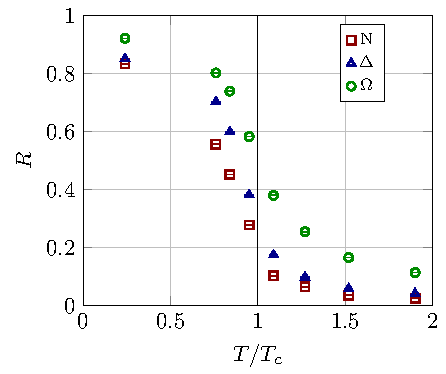
\includegraphics[width=0.83\textwidth]{figures/baryon_plot.pdf}
  \end{center}

\end{frame}

\begin{frame}[plain]
  \begin{center}
    {\changefontsize{36pt}\color{Tropiteal}Thanks!}
  \end{center}
\end{frame}

\end{document}
